%(BEGIN_QUESTION)
% Copyright 2010, Tony R. Kuphaldt, released under the Creative Commons Attribution License (v 1.0)
% This means you may do almost anything with this work of mine, so long as you give me proper credit

Anta at et voltmeter viser 0 volt mellom testpunktene {\bf A} og {\bf D}, og også 0 volt mellom testpunktene {\bf A} og {\bf G}:

$$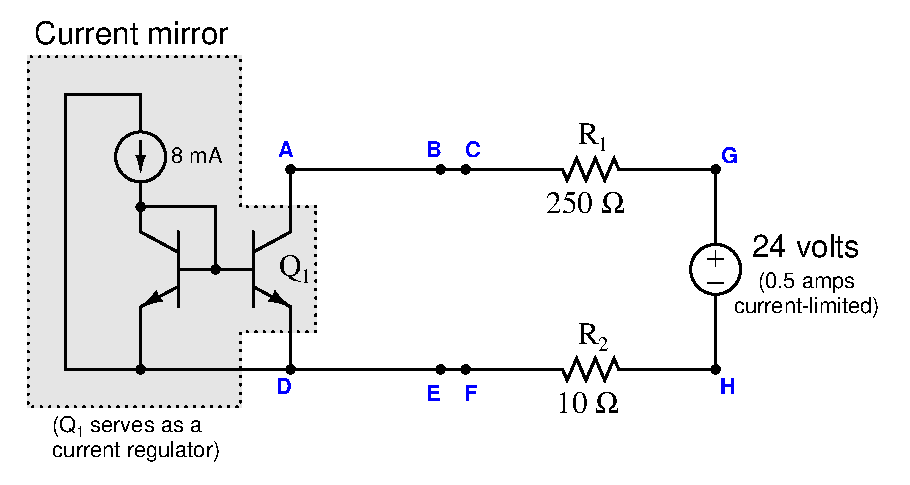
\includegraphics[width=15.5cm]{i00439x01.eps}$$

Vurder sannsynligheten for hver oppgitt feil i denne kretsen. Se på én feil om gangen (ingen samtidige feil), og avgjør om hver feil alene kan forklare {\it alle} målinger og symptomer i kretsen.

% No blank lines allowed between lines of an \halign structure!
% I use comments (%) instead, so that TeX doesn't choke.

$$\vbox{\offinterlineskip
\halign{\strut
\vrule \quad\hfil # \ \hfil & 
\vrule \quad\hfil # \ \hfil & 
\vrule \quad\hfil # \ \hfil \vrule \cr
\noalign{\hrule}
%
% First row
{\bf Feil} & {\bf Mulig} & {\bf Umulig} \cr
%
\noalign{\hrule}
%
% Another row
$R_1$ avbrudd &  &  \cr
%
\noalign{\hrule}
%
% Another row
$R_2$ avbrudd &  &  \cr
%
\noalign{\hrule}
%
% Another row
$Q_1$ avbrudd &  &  \cr
%
\noalign{\hrule}
%
% Another row
$R_1$ kortsluttet &  &  \cr
%
\noalign{\hrule}
%
% Another row
$R_2$ kortsluttet &  &  \cr
%
\noalign{\hrule}
%
% Another row
$Q_1$ kortsluttet &  &  \cr
%
\noalign{\hrule}
%
% Another row
Spenningskilde død &  &  \cr
%
\noalign{\hrule}
%
% Another row
Strømkilde død &  &  \cr
%
\noalign{\hrule}
} % End of \halign 
}$$ % End of \vbox

Angi til slutt hvilken {\it neste} diagnostiske test eller måling du ville gjort på systemet. Forklar hvordan resultatet av denne testen hjelper videre med å identifisere feilsted og/eller feiltype.

\vfil 

\underbar{file i00439}
\eject
%(END_QUESTION)





%(BEGIN_ANSWER)

Dette er en vurderingsoppgave, så her gis ingen svar eller hint.

%(END_ANSWER)





%(BEGIN_NOTES)

0 volt mellom punkt A og D (isolert sett) kan bety enten avbrutt strømtilførsel til transistoren, eller at $Q_1$ er kortsluttet. Men 0 volt mellom A og G utelukker kortsluttet $Q_1$ (ved enkeltfeil), fordi kortsluttet $Q_1$ ville gitt spenningsfall over $R_1$. Målingen A-G = 0 volt utelukker også avbrudd i $R_1$.

Ingen av motstandene kan være kortsluttet, fordi det ville gitt spenning over transistoren. Avbrudd i $Q_1$ ville på samme måte gitt spenning mellom A og D. Død strømkilde ville gjort $Q_1$ ikke-ledende (åpen), noe som ikke kan stemme siden spenningsfallet mellom A og D er 0.

Da gjenstår bare avbrudd i $R_2$ eller død spenningskilde som mulige feil.

% No blank lines allowed between lines of an \halign structure!
% I use comments (%) instead, so that TeX doesn't choke.

$$\vbox{\offinterlineskip
\halign{\strut
\vrule \quad\hfil # \ \hfil & 
\vrule \quad\hfil # \ \hfil & 
\vrule \quad\hfil # \ \hfil \vrule \cr
\noalign{\hrule}
%
% First row
{\bf Feil} & {\bf Mulig} & {\bf Umulig} \cr
%
\noalign{\hrule}
%
% Another row
$R_1$ avbrudd &  & $\surd$ \cr
%
\noalign{\hrule}
%
% Another row
$R_2$ avbrudd & $\surd$ &  \cr
%
\noalign{\hrule}
%
% Another row
$Q_1$ avbrudd &  & $\surd$ \cr
%
\noalign{\hrule}
%
% Another row
$R_1$ kortsluttet &  & $\surd$ \cr
%
\noalign{\hrule}
%
% Another row
$R_2$ kortsluttet &  & $\surd$ \cr
%
\noalign{\hrule}
%
% Another row
$Q_1$ kortsluttet &  & $\surd$ \cr
%
\noalign{\hrule}
%
% Another row
Spenningskilde død & $\surd$ &  \cr
%
\noalign{\hrule}
%
% Another row
Strømkilde død &  & $\surd$ \cr
%
\noalign{\hrule}
} % End of \halign 
}$$ % End of \vbox


%INDEX% Troubleshooting review: electric circuits

%(END_NOTES)
